\documentclass{./../div_teaching_slides}
\begin{document}

\title{ECON 340 \\ Economic Research Methods}
\author{Div Bhagia \\\vspace{1.75em}
Lecture 5 \\\vspace{0.25em} \small Research Questions and Data}
\date{}

%%%%%%%%%%%%%%%%%%%%
\begin{frame}[noframenumbering, plain]
\maketitle
\end{frame}

%%%%%%%%%%%%%%%%%%%%
\begin{frame}{Discussion: Chapter 1, Stock and Watson}
1. Does reducing class size improve elementary school education? \\ \vspace{0.5em}
\begin{witemize}
  \item Using data on 420 California school districts in 1999, we find that \textit{students in districts with small class sizes tend to perform better on standardized tests.}
  \item Can we conclude that small class sizes $\rightarrow$ better test scores?
  \item What could be some \textit{confounding} factors?
\end{witemize}
\end{frame}

%%%%%%%%%%%%%%%%%%%%
\begin{frame}{Discussion: Chapter 1, Stock and Watson}
2. Is there racial discrimination in the market for home loans? \\ \vspace{0.5em}
\begin{witemize}
  \item Researchers at the Federal Reserve Bank found that 28\% of black applicants are denied mortgages, while only 9\% of white applicants are denied.
  \item Does this indicate there is racial bias in mortgage lending?
  \item What could be some \textit{confounding} factors?
\end{witemize}
\end{frame}

%%%%%%%%%%%%%%%%%%%%
\begin{frame}{Discussion: Chapter 1, Stock and Watson}
3. Does healthcare spending improve health outcomes? \\ \vspace{0.5em}
\begin{witemize}
  \item What are the two challenges identified in the reading when trying to answer this question using cross-country data on healthcare expenditures and mortality rates? 
\end{witemize}
\end{frame}

%%%%%%%%%%%%%%%%%%%%
\begin{frame}{Discussion: Chapter 1, Stock and Watson}
4. By how much will US GDP grow next year? \\ \vspace{0.5em}
\begin{witemize}
  \item How is this question different from the first three? 
\end{witemize}
\end{frame}

%%%%%%%%%%%%%%%%%%%%%
%\begin{frame}{Today's Agenda}
%\begin{witemize}
%\item Types of questions: causality vs. prediction
%\item Types of data and variables
%\item What questions can you answer, and where to start? \\~\\
%\end{witemize}
%Reference:
%\begin{witemize}
%\item Chapter 1 from Stock and Watson's Introduction to Econometrics textbook (uploaded on Canvas) 
%\end{witemize}
%\end{frame}

%%%%%%%%%%%%%%%%%%%%%
%\begin{frame}{Types of Questions}
%Let's consider the following questions: \\~\\
%\begin{witemize}
%  \item Does the use of electronic devices inhibit classroom learning? \\
%  \item Who will win the next US election? \\~\\
%\end{witemize}
%\pause The first question concerns a \textit{causal} relationship between the use of phones and classroom learning. \\~\\
%While the second one is about \textit{predicting} an outcome.
%\end{frame}

%%%%%%%%%%%%%%%%%%%%
\begin{frame}{Causal Questions}
\begin{witemize}
  \item Causality: specific action leads to specific, measurable consequences 
  \item The first three questions we discussed are causal
  \item More examples:\\
  \begin{witemize}
  \normalsize
  \item Does sleep affect productivity?
  \item Will the Fed's interest rate hike lower inflation?
  \item Do higher minimum wages decrease employment?
\end{witemize}
\end{witemize}
\end{frame}

%%%%%%%%%%%%%%%%%%%%
\begin{frame}{Prediction}
\begin{witemize}
  \item Prediction: using the information on some variables to predict the value of another variable
  \item You do not need to know a causal relationship to make a good prediction
  \item A good way to ``predict'' whether it is raining is to observe whether pedestrians are
using umbrellas, but using an umbrella does not cause it to rain.
\item Forecasting: predictions about the future
\end{witemize}
\end{frame}

%%%%%%%%%%%%%%%%%%%%
\begin{frame}{Where are we headed?}
\begin{witemize}
  \item Conceptual framework we will build up to in this class---multiple regression model 
  \item Multiple regression model can be used to answer both types of questions 
  \item The multiple regression model is very useful because it gives us a mathematical way to \textit{quantify how a change in one variable affects another variable, holding other things constant}.
  \item You will be utilizing this model for your research project
\end{witemize}
\end{frame}

%%%%%%%%%%%%%%%%%%%%
\begin{frame}{Multiple Regression Model}
 For example, using the multiple regression model, we can answer questions such as: \\ \vspace{0.5em}
\begin{witemize}
\item[] What effect does a change in class size have on test
scores, holding constant or \textit{controlling} for student characteristics (such as family
income)? 
\item[] What effect does your race have on your chances of having a mortgage application granted, holding constant other factors such as your ability to repay the loan?
\end{witemize}
\end{frame}


%%%%%%%%%%%%%%%%%%%%
\begin{frame}{Dependent vs Independent Variable}
\begin{witemize}
  \item The outcome variable is often called the \textit{dependent variable}
  \item The variable(s) that affect the dependent variable are called \textit{independent variable}(s)
  \item Other variables that might confound the effect of an independent variable on the dependent variable are called \textit{control variables}
\end{witemize}
\end{frame}


%%%%%%%%%%%%%%%%%%%%
\begin{frame}{Your Research Project}
\begin{witemize}
\item Pick a question that can be answered using one of the datasets compiled for this class or an external dataset
\item The question should be \textit{well-defined} and \textit{feasible} using the data you picked \\~\\ 
\end{witemize}
Not well-defined: \textit{Are smaller classes better?} \\~\\
Well-defined: \textit{Does a smaller class size lead to better scores on standardized tests?}
\end{frame}

%%%%%%%%%%%%%%%%%%%%
\begin{frame}{Your Research Project}
\vspace{-0.5em}
Say, you picked this question: \textit{Does a smaller class size lead to better scores on standardized tests?} \\ \vspace{0.25em}
\begin{witemize}
\item Identify your dependent variable
\item Identify your independent variable
\item Identify some other variables in the dataset that are potential confounders, which will be your control variables. \\  \vspace{0.5em}
\end{witemize}
If all the needed variables are available in your dataset, your question is feasible. \\ \vspace{0.5em}
%This will be your task for the first research project submission.
\end{frame}

\begin{frame}{Types of Data}
Experimental versus observational (mostly what we will use) \\~\\
\begin{witemize}
\item \textbf{Cross-Sectional:} many entities, single time period
\item \textbf{Time Series:} single entity, multiple time periods 
\item \textbf{Panel/Longitudinal Data:} multiple entities, multiple time periods \\~\\
\end{witemize}
Examples?
\end{frame}

%%%%%%%%%%%%%%%%%%%%
\begin{frame}{Establishing Causality}
\begin{witemize}
  \item As we have said, establishing causality is hard. 
  \item Think about the following question: \\ \vspace{0.5em}
  \textit{Does the use of electronic devices inhibit classroom learning?}
  \item Say, I give you data from all classes held at CSUF in the last five years. The data contains average grades for each class and whether the instructor allowed electronic devices in the classroom. 
  \item Could you answer the above question? If yes, how?
\end{witemize}
\end{frame}

%%%%%%%%%%%%%%%%%%%%
\begin{frame}{Establishing Causality}
\begin{witemize}
\item We could compare grades for classes in which devices are permitted vs. others
\item But what if better instructors don't care about students using devices?
\item This would lead us to find little impact of device use, as classes where devices are allowed also happen to be taught by better instructors
\item Here, the instructor quality is an example of a \textit{confounding} factor
\end{witemize}
\end{frame}

%%%%%%%%%%%%%%%%%%%%
\begin{frame}{Establishing Causality}
\begin{witemize}
\item How to establish causality? \\
\begin{itemize}
\item\normalsize Gold standard: experiments/randomized controlled trials (RCTs)
\item Assign randomly to \textit{treatment} or \textit{control} group 
 \end{itemize} 
 \item Carter, Greenberg, and Walker (2017): randomly allowed students to access their laptop and tablet computers during an introductory economics course at the United States Military Academy at West Point
\end{witemize}
\end{frame}

%%%%%%%%%%%%%%%%%%%%
\begin{frame}{Carter, Greenberg, and Walker (2017)}
 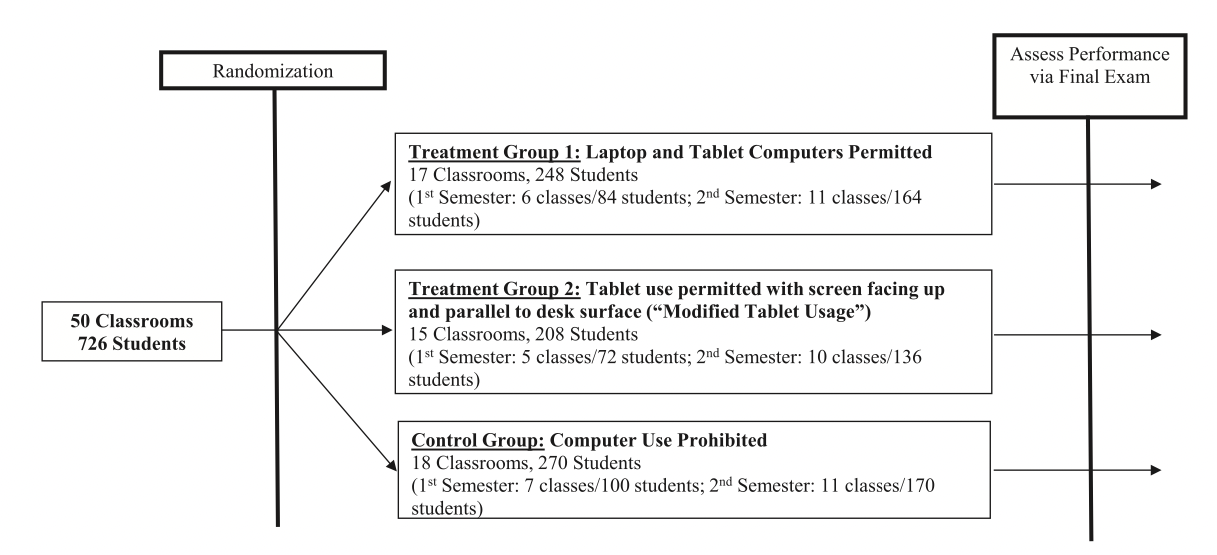
\includegraphics[scale=0.35]{exp.png}
\end{frame}

%%%%%%%%%%%%%%%%%%%%
\begin{frame}{Why does randomization help?}
\begin{witemize}
  \item Which classes allow electronic devices or not is random
  \item There should be no differences in instructor effectiveness because the classes were chosen randomly
  \item RCTs are widely employed in clinical research, e.g., experimental drug trials, other treatments
  \item Increasingly used in economics and other social sciences, e.g., PROGRESSA, free deworming program in Kenya (Miguel and Kremer, 2004), microcredits (Banerjee et al., 2013)
\end{witemize}
\end{frame}

%%%%%%%%%%%%%%%%%%%%
\begin{frame}{\large Aside: Experiments in Development Economics}
\begin{witemize}
  \item Development economists were early adopters of experiments in economics
  \item The 2019 Nobel prize in economics was awarded to Abhijit Banerjee, Esther Duflo, and Michael Kremer ``for their experimental approach to alleviating global poverty.''
  \item (Duflo is the youngest person and the second woman to win the award.)
  \item If you are intrigued, check out Poor Economics by Banerjee and Duflo
\end{witemize}
\end{frame}

%%%%%%%%%%%%%%%%%%%%
\begin{frame}{But, we can't all run experiments...}
\begin{witemize}
\item Hard to conduct experiments for a lot of Economics questions
\item Economists have developed a whole toolkit of \textit{quasi-experimental} methods. This is the heart of Econometrics.  
\item Starting point: multiple regression model that allows us to \textit{control} for variables
\item Focus on being able to come as close as possible to an idealized experiment
\end{witemize}
\end{frame}

%%%%%%%%%%%%%%%%%%%%
\begin{frame}{Another aside}
\begin{witemize}
  \item The 2021 Nobel prize in economics was awarded to David Card, Joshua D. Angrist, and Guido W. Imbens for their contributions to answering causal questions using \textit{natural experiments}
  \item In the last two decades, \textit{quasi-experimental} methods have been used to quantify the labor market effects of minimum wages, immigration, and education, amongst other questions. 
  \item We will talk more about this towards the end of the semester.
\end{witemize}
\end{frame}

%%%%%%%%%%%%%%%%%%%%%
%\begin{frame}{Some Sources of International Data}
%\begin{witemize}
%\item World Bank: large datasets across countries, including the World Development Indicators (WDI) database and the Global Financial Development Database (GFDD)
%\item United Nations Statistic Division: international economic, health, education, and development data
%\end{witemize}
%\end{frame}
%
%%%%%%%%%%%%%%%%%%%%%
%\begin{frame}{Some Sources of US Economic Data}
%\begin{witemize}
%\item FRED at the Federal Reserve Bank of St. Louis maintains numerous data series
%\item US Bureau of Labor Statistics (BLS): labor-related statistics such as wage and employment data
%\item US Bureau of Economic Analysis (BEA): economic variables for US states
%\item County Business Patterns Data from the US Census
%\end{witemize}
%\end{frame}
%
%%%%%%%%%%%%%%%%%%%%%
%\begin{frame}{Some Sources of US Micro Data}
%\begin{witemize}
%\item IPUMS: to download US microdata
%\begin{itemize}
%\normalsize
%\item Current Population Survey (CPS), 
%\item American Community Survey (ACS),
%\item American Time-Use Survey (ATUS), etc.
%\end{itemize}
%\item US longitudinal datasets: 
%\begin{itemize}
%\normalsize
%\item Panel Study of Income Dynamics (PSID)
%\item National Longitudinal Surveys (NLSY)
%\end{itemize}
%\end{witemize}
%\end{frame}

%%%%%%%%%%%%%%%%%%%%%
%\begin{frame}{What is a variable?}
%\begin{witemize}
%\item A \textit{variable} is multiple observations of the same measurement \\~\\
%\begin{witemize}
%\normalsize
%\item Daily rainfall for the last 100 years 
%\item Annual income of all US adults
%\item Gender of everyone in this classroom
%\item List of all books on The New York Times bestseller list
%\end{witemize}
%\end{witemize}
%\end{frame}
%
%%%%%%%%%%%%%%%%%%%%%
%\begin{frame}{Types of Variables}
%\begin{witemize}
%\item \textit{Continuous}: income, age, GPA
%\item \textit{Count}: classes this semester, how many days did it rain last year
%\item \textit{Ordinal}: high, low, medium; education level
%\item \textit{Categorical}: gender, race, religious affiliation
%\item \textit{Binary}: categorical variable with two categories
%\item \textit{Qualitative}: everything else 
%\end{witemize}
%\end{frame}


%%%%%%%%%%%%%%%%%%%%
\begin{frame}{Things To Do Next}
\vspace{-0.5em}
\begin{witemize}
\item For the rest of this week and next week, we will learn how to prepare and analyze data in R
\item Install R and R Studio on your computer if you haven't (how to handout on Canvas)
\item Download the dataset ``caschool.csv'' from our \href{https://www.dropbox.com/sh/9x7ac4qwnddl650/AAAP1FdTpFp2rXyZ6t-9-qqTa?dl=0}{Dropbox data folder} and save it in a new folder called ``Econ340\_R'' on your laptop (don't forget the location of the folder).
\item Bring your laptop to the next class. Alternatively, you can use the computers in the lab. In the latter case, try to be here 5 minutes before class to set up.
\end{witemize}
\end{frame}

\end{document}